\section{Literature review}
\subsection{Structure of the thesis}

The thesis comprises the front matter, the main matter and possible appendices.
The front matter in the required order is:

%% An example of an unordered (itemised) list with the default bullet point
%% label.
\begin{itemize}
	\item a cover page,
	\item a page containing copyright information,
	\item the abstract page(s),
	\item an optional preface, and
	\item a table of contents.
\end{itemize}

If the thesis contains mathematical equations, give the list of symbols used to 
represent various quantities along with the mathematical operators used.
The list must contain all the abbreviations used as well. Note that lists of
figures and tables are not required.

The main matter, i.e. the actual thesis, begins after the list of symbols and 
abbreviations. Its structure follows the standard structure used in scientific 
writing. A typical division of the content is
%% An example of an ordered (numbered) list with the default numbering.
\begin{enumerate}
	\item \label{list:intro} Introduction (research objectives and questions)
	\item Literature review (research made earlier in this area)
	\item Research material and methods
	\item Results / Findings
	\item Discussion
	\item \label{list:summary} Summary / Conclusions
	\item References
\end{enumerate}
The parts \ref{list:intro}--\ref{list:summary} in the list above are the text  
of your thesis. Often the discussion and summary (or conclusions) are combined 
in one chapter. The wording of the titles suggested above may differ. As a 
matter of fact, the titles above refer more to the type of content rather than 
being title suggestions. For example, the literature review of a thesis on 
electromagnetics could be under the title ‘Electromagnetic theory and FDTD’. 
The background to the methodology used---FDTD here---could also be in this 
chapter. Note that the chapters and sections within the main matter are 
numbered, and that they appear in the table of contents. The references, or the 
bibliography, is also shown in the table of contents, but without a number 
labelling it.

The appendix or appendices, when necessary, are presented in the last part of
the thesis. They contain things like questionnaires used in the study, 
[selected parts of] data, derivations of mathematical results, a more detailed 
exposition of some aspect in the thesis, or code listings. Number them in the 
table of contents as follows:
%% An example of an ordered list with the capital-letter numbering. The letter
%% nubering is limited to this list only.
\begin{enumerate}
\renewcommand{\labelenumi}{\Alph{enumi}.}
	\item The first appendix
	\item The second appendix
\end{enumerate}

Refer to a suitable guide on writing a thesis for a comprehensive description;
there are plenty of them around. The instructions here are not exhaustive, and
they concentrate more on how to use this template.

A bachelor’s thesis is ideally about 20 pages long, excluding the appendices, 
whereas a master’s thesis is about 60 pages long, again, not counting the pages
in the appendices. The numbers pertaining to the length of your thesis given
here are mere rules of thumb. Consult your school’s thesis guidelines and your 
thesis advisor and/or supervisor for the appropriate length in your case.


\subsection{Page numbering}
Number the pages using Arabic numerals, placed in the centre of the page footer.
The numbering begins from the cover page and runs continuously to the end of the 
thesis. Enter the total number of pages in the thesis---front matter, main
matter and appendices, if present---in the appropriate field on the abstract
page. Enter also the number of pages in the appendices, if present, in the same 
field on the abstract page as follows: total number of thesis pages / number of 
pages in the appendices.

Do not print the page numbers on the cover and the copyright pages; number all
the other pages. Thus, the first page with a page number printed on it---the
first abstract page---is ‘3’. The page numbering of appendices continues from
that on the previous page.


\subsection{Structuring the text in the main matter}
\subsubsection{Sections}

You can structure your text by dividing it into sections with a suitable title. 
Well-devised sectioning clarifies your text, but beware of overusing them, since 
that will fragment and confuse your text. Do not use more than three levels of 
hierarchy in your sections. Notice that the section titles, just as the figure
and table labels, are in a Helvetica clone, a sans serif, or grotesque, font. 
The main matter text is typeset in a Times clone, a serif font.

The sectioning macros available in \LaTeX{} are 
%% \section{title} 
%% \subsection{subtitle}
%% \subsubsection{subsubtitle}
\begin{itemize}
	\setlength{\itemsep}{0pt}
	\item[] \verb+\section{title}+,
	\item[] \verb+\subsection{subtitle}+, and
	\item[] \verb+\subsubsection{subsubtitle}+.
\end{itemize}

The formatting specifications are in appendix~\ref{app:layout}. The fonts 
specified there are for Word documents, as specified by Aalto's visual 
guidelines. No corresponding fonts are officially specified for \LaTeX{}. Hence,
similar corresponding fonts provided by the \verb+newtxtext+ package are used in
this template. Math fonts are those from \verb+newtxmath+. The most important 
factor that influenced this choice of fonts was that the package outputs 
PDF/A-1b compliant pdf using \texttt{pdflatex}.

At least in technical texts, refraining from using the articles ‘a’ and ‘the’ as
the first word in the title is common practice. Appendices are enumerated using 
capital letters. Begin every section on a new page. Begin a subsection on a new 
page only if the previous page is full. Similarly, begin every appendix on a new
page.

\subsubsection{Paragraphs}

The paragraph that follows the section title is not indented, the paragraphs 
that follow are. Often, the body text is typeset as raggedright to avoid 
unnecessarily large white spaces between words. On the other hand, in many 
technical fields, the text is justified on both sides, but in such cases, 
hyphenation is used to maintain reasonable separation between words. This 
template uses justified text with automatic hyphenation. Write paragraphs so 
that they span more than three lines. Rethink your text, if you end up having  
one-line paragraphs; avoid them in your thesis---including the appendices. In 
addition, you may need to reconstruct your text if your paragraphs are too long.
Avoid emphasising text using italics. Italicised text makes reading for dyslexic
readers even more difficult.

When a number has a unit associated with it, ensure two things: the space 
between the number and the unit is smaller than the regular space (for example, 
1\,Hz) and the number and unit are not split over lines. You can simply use 
\verb+\,+ between the number and the unit without spaces between them to stop 
them from being split (\verb+1\,Hz+) or use the package \verb+siunitx+.


\subsubsection{Equations}

Equations are numbered using Arabic numerals, typically enclosed in parentheses,
but not always. This template encloses equation numbers in parentheses. An 
example equation is
\begin{equation}
	f(x) = a_0 + \sum_{n=1}^{\infty} \left( a_n \cos\frac{n\pi x}{L} + 
	b_n \sin\frac{n\pi x}{L} \right).
\end{equation}
Closely related equations like equations in a system of equations may be numbered 
as follows:
\begin{subequations}\label{eq:ohm}
  \begin{alignat}{1}
	V_\text{s} &= R_\text{s} i_\text{s} + R(i_\text{s} + i_\text{b})
	 \label{eq:ohm1}\\
	V_\text{b} &= R_\text{b} i_\text{b} + R(i_\text{b} + i_\text{s}).
	 \label{eq:ohm2}
  \end{alignat}
\end{subequations}
All equations need not be numbered. Remember punctuation after the equation; an
equation is an integral part of your sentence and may need to be followed by 
punctuation marks. Many scientific journals do not use them after equations;
then again, many do. Punctuate the equations in your thesis. Numbering of
equations in appendices consists of the appendix numbering alphabet followed by
the equation number, which starts from one in each appendix. For example, the
first equation in appendix A would be equation~(A1) and the first two 
equations~(A1)--(A2).

\subsubsection{Figures and tables}

Theses generally contain figures and tables, which have captions describing 
them. For figures, the convention is to place the caption after (below) the 
figure, as shown in figure~\ref{fig:coil} and figure~\ref{fig:graph}. Tables, on
the other hand, have the caption above (before), as evident from 
table~\ref{tab:animals}. The label and number are typeset in the sans serif bold
12-pt typeface and the caption in the serif 12-pt normal typeface (see 
appendix~\ref{app:layout}).

%% Example of a figure
%% The environent's optional arguments h (here), t (top), b (bottom) and p
%% (page) try to force LaTeX to place the figure as directed as opposed to being
%% place there where LaTeX deems appropriate. 'p' places the figure on the next
%% page by itself. The order of the arguments determines the preference that is
%% desired. These arguments apply to the table environment as well.
\begin{figure}[tb]
  \centering
  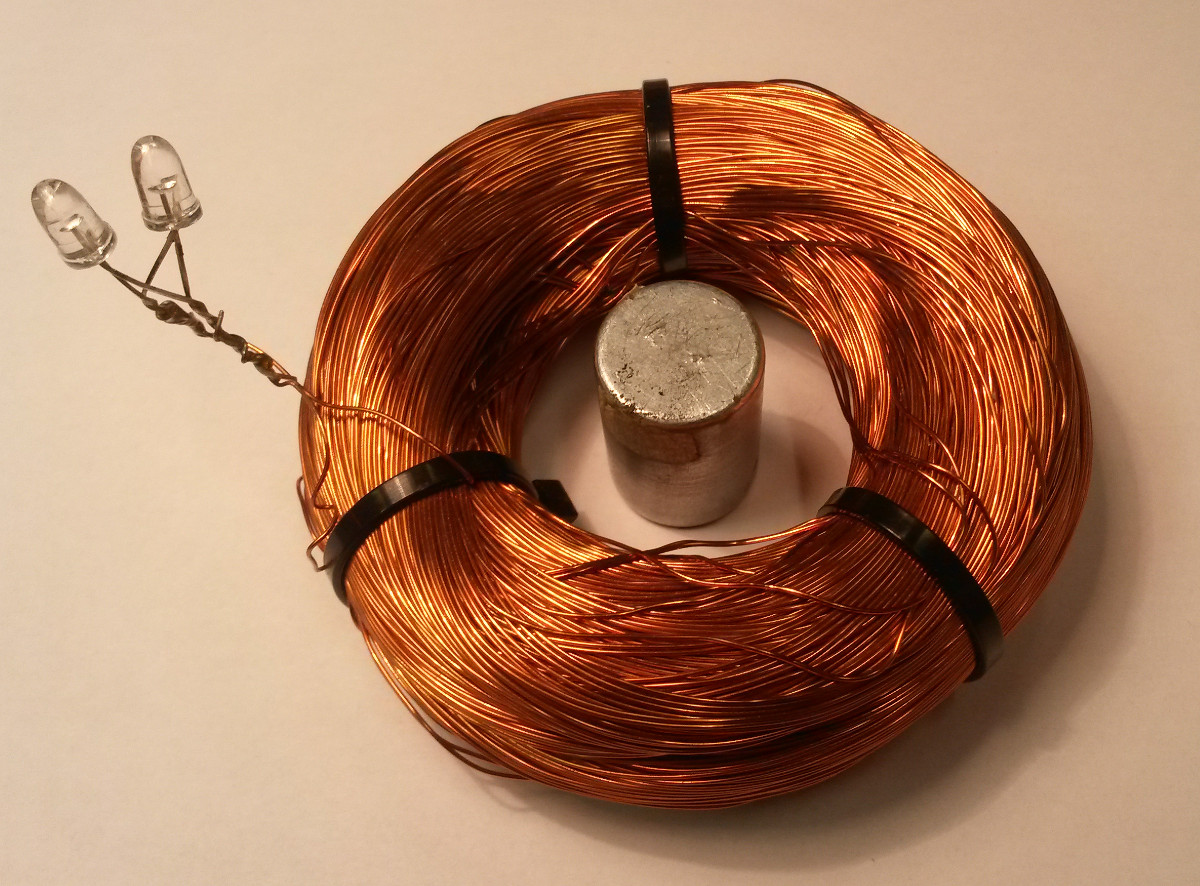
\includegraphics[alt={A coil of copper wire with a magnet placed in the centre of the coil and two LEDs connected at the ends of the coiled wire.}, height=5cm]{./images/ledspole.jpg}
  \caption{A coil terminated in two LEDs with a magnet placed at its centre!!}
  \label{fig:coil}
\end{figure}

\begin{figure}[tb]
  \centering
  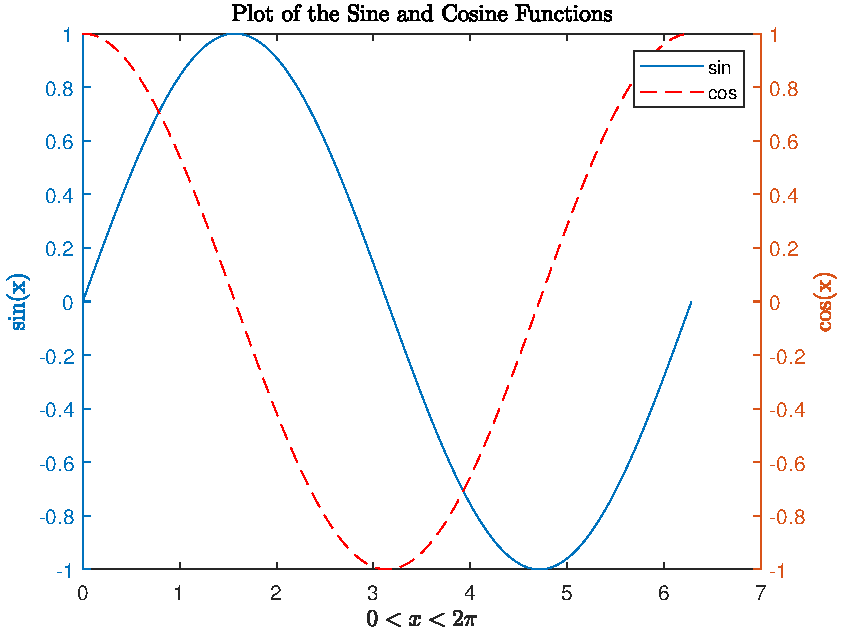
\includegraphics[alt={One period of a since and a cosine curve from 0 to 2 pi radians and having amplitude 1.}, height=5cm]{./images/curves.pdf}
  \caption{Example of a MATLAB graph.}
  \label{fig:graph}
\end{figure}

%% Example of a table
\begin{table}[tb]
	\centering
	\caption{An example table. Common animals classified into their classes.}
	\label{tab:animals}
	\sffamily% change the font in the table to sans serif
	\begin{tabular}{ccc}
	  \hline
	  \textbf{Mammals} & \textbf{Birds} & \textbf{Insects}\\ \hline
	  dog & crow & ladybird \\ \hline
	  cat & sparrow & ant \\ \hline
	  rat & tit & cockroach \\ \hline
	\end{tabular}
\end{table}

Avoid placing figures and tables such that they are preceded or followed by just
a line or two, because the reader can have difficulties in finding the line(s) 
of text and might even accidentally miss the text completely. Consider, for 
example, a page beginning with one line of text continued from the preceding 
page and that ends the paragraph. This is followed by a figure, then a short 
three-line paragraph, then yet another figure, followed by more text, which is 
positioned such that only two lines of text are on the page and the remainder is
placed on the following page. The layout of this page is fragmented, and as a 
result, the reader might initially miss the top line of text. Consider using one
of the following three layout possibilities: place the figures in the top part 
of the page followed by the text, or place the text in the top followed by the 
figures, or place all the text in the middle with one figure on the top and the 
other at the bottom. Base your choice on considering how easily the reader can 
follow your text (the content of the figures affects this), and whether the page
as a whole looks ordered and pleasing to the eye.

Strive to place the referenced figure or table on the same page as where it is 
referenced. If this is difficult, place it on the following page, but not very 
much further. Using the options \texttt{b} (for bottom), \texttt{t} (for top), 
\texttt{h} (for here) and \texttt{p} (for separate page) judiciously in the 
\texttt{figure} and \texttt{table} environments, \LaTeX{} does a pretty good 
job of placing figures and tables. However, placing figures (and tables) close 
to where they are referred to may be impossible when you have many pictures, so 
use common sense and keep the reader in mind when placing pictures and tables.


\subsection{Referencing parts in the thesis}

Cross-referencing in \LaTeX{} is simple and straightforward: use 
\verb+\label{marker}+ to label the object with a number and then refer to the 
object using \verb+\ref{marker}+. \texttt{marker} should be a unique string of 
characters. To help keep you organised with the various reference labels, be 
systematic when creating them for different objects in the thesis. For example, 
start labels for figures with \texttt{fig:}, for tables with \texttt{tab:}, 
\texttt{sec:} for sections, and \texttt{eq:} for equations, as done in this 
template. So, you could have, say, \verb+\label{sec:ohmslaw}+, 
\verb+\label{eq:ohmslaw}+, \verb+\label{fig:ohmslaw}+, and 
\verb+\label{tab:ohmslaw}+.

Perhaps you will have noticed that when referencing objects in the text, as is 
done for `figure' earlier in the text, the label ‘figure’ in the cross-reference
is not capitalised. Often, you see the capitalised label ‘Figure’. In such 
cases, the label together with the number, for example ‘Figure 2’, is 
considered a proper noun, hence the capitalisation. Although this template uses 
the lowercase form, you can choose how you write cross-referencing labels: 
‘figure’ or ‘Figure’---you will do well to consult your advisor and supervisor 
about this; they may have strong opinions on the matter. However you decide to 
write cross-referencing labels---figure, table, section or equation---be 
consistent.

Do not abbreviate any of the labels, for example ‘figure’ to ‘fig.’ or ‘Fig.’. 
Journals do this because the amount of available space for an article is 
limited; space is not an issue in your thesis. You can refer to more than one 
figure, for example, by saying figures~\ref{fig:coil} and \ref{fig:graph}. Use 
endash `\verb+--+' to specify a range: sections~\ref{sec:intro}--\ref{sec:summary}.

To reference a section, place the section label directly after the sectioning 
command of the section to be referenced. For example:
%% The verbatim environment typesets text within it as-is. Commands are not
%% interpreted and executed within the environment.
\begin{verbatim}
	\subsection{Ohm's law}
	\label{sec:ohmslaw}
	...
	...as discussed in section~\ref{sec:ohmslaw}, the resistance...
\end{verbatim}
The tilde placed between `section' and `\verb+\ref{sec:ohmslaw}+' not only puts 
a normal space between the two, but also binds them so that they are not split 
over separate lines if the two occur at the end of a line. Put a tilde between 
all labels and the reference number.

For figures and tables, place the label text after \verb+\caption+. For simple 
equations, the label is placed after \verb+\begin{equation}+. You can reference
individual items such as equation~(\ref{eq:ohm1}) in a grouped equation 
enviroment like \verb+subequations+ or an item in an itemised list like 
item~\ref{list:intro} on page~\pageref{list:intro} or the system of 
equations~(\ref{eq:ohm}) by putting a \verb+\label+ appropriately.

\subsection{Citation}

The list of reference must be carefully made, following one of many different 
styles. Which you choose depends on the field of your thesis. However, citing 
using footnotes is not allowed in your thesis\footnote{Adding comments in 
footnotes is \underline{not} allowed either.}. A short reference list can have 
entries in the order in which they are cited, but if your list is long, arrange 
the entries in alphabetical order. Read appendix~\ref{app:reference} for a 
fairly thorough discussion of how to cite work in academic writing and make a 
bibliography or list of references. Remember that referencing is a very 
important part of your thesis, so be meticulous and thorough.

\subsubsection{Bibliography or list of references}

Find here a list of some of the typical entries in the bibliography and the 
information they must contain. For a more comprehensive list, see 
\cite{aaltolib}. See appendix~\ref{app:reference} for details on how this 
information must be typeset in different reference styles.\\

\noindent
A \underline{book} entry must contain the following:
\begin{itemize}
\setlength{\itemsep}{-3pt}
\item[--]author(s) 
\item[--]title of the book
\item[--]edition, if there are more than one
\item[--]publisher
\item[--]place of publication
\item[--]time of paublication (typically year)
\item[--]name of series, if the book is part of a series
\end{itemize}
References \cite{Kauranen}--\cite{Koblitz} are examples of books in the 
bibliography. Refering to a particular place in a book, for example like this, 
\cite[s.\ 83--124]{Koblitz}, is a good practice. The reader can thus find the 
referred matter easily.\\

\noindent
The following must be found in an \underline{article} entry:
\begin{itemize}
	\setlength{\itemsep}{-3pt}
\item[--]author(s)
\item[--]title of the article
\item[--]name of the journal or magazine where the article is published
\item[--]volume number of the journal or magazine
\item[--]issue number of the journal or magazine
\item[--]year of publication
\item[--]page numbers of the published article
\end{itemize}
References \cite{bcs}--\cite{Deschamps} are examples of articles in a 
bibliography.\\

\noindent
An \underline{edited book} or \underline{compilation} of contributions, 
typically chapters or articles, from several authors having one or more editors 
or a compiled conference proceedings must have the following information:
\begin{itemize}
\setlength{\itemsep}{-3pt}
\item[--]author(s) of the chapter or part
\item[--]title of the chapter or part
\item[--]mention the kind of publication `In book', or for conference 
proceedings with no editor information use `In' before the name of the 
conference proceedings
\item[--]editor(s) of the compilation identified with (Ed.) or (Eds.)
\item[--]name of the compiled book or conference
\item[--]for a conference article, the time and place where the conference was 
held
\item[--]edition, if more than one
\item[--]place of publication
\item[--]publisher (may not exist for conference proceedings)
\item[--]time (year) of publication
\item[--]pages of cited contribution
\item[--]name of series, if the book is part of one
\end{itemize}
References \cite{Sihvola}--\cite{Lindblom} are examples of references to a part 
of a compilation.\\

\noindent
\underline{Theses} must have the following information:
\begin{itemize}
\setlength{\itemsep}{-3pt}
\item[--]author
\item[--]title of the thesis
\item[--]type of thesis (bachelor's, master's doctoral, other)
\item[--]name of university or institution
\item[--]name of the department, faculty or degree programme
\item[--]location/place of the university or institution
\item[--]year of publication
\end{itemize}
References \cite{Miinusmaa}--\cite{Lonnqvist} are examples of theses in a 
bibliography.\\

\noindent
\underline{Standards} must have the following:
\begin{itemize}
\setlength{\itemsep}{-3pt}
\item[--]standard identifier and number
\item[--]name of the standard
\item[--]edition, if not the first
\item[--]place of publication
\item[--]publisher
\item[--]year of publication
\item[--]number of pages
\end{itemize}
Reference \cite{sfs} is an example of how a standard is entered in a 
bibliography.\\

\noindent
An \underline{interview} entry must have the following details:
\begin{itemize}
\setlength{\itemsep}{-3pt}
\item[--]name of the interviewee
\item[--]position or t academic and/or professional title
\item[--]organisation where the interviewee is placed
\item[--]address of the organisation
\item[--]a mention that the entry is an interview along with the date of the 
interview
\end{itemize}
Reference \cite{interview} is an example of an interview entry in a 
bibliography.

Most scientific articles are available online nowadays and many also in printed 
form. Articles from journals, magazines or other publications available 
\underline{only online} must have the following details in the bibliography:
\begin{itemize}
\setlength{\itemsep}{-3pt}
\item[--]author(s)
\item[--]name of the article
\item[--]name of the publication (journal or magazine)
\item[--]type of publication
\item[--]edition or volume
\item[--]volume number and issue details of publication and article
\item[--]year of publication along with details on possible updates: Updated, 
date of update
\item[--]mention `Accessed' and date when accessed
\item[--]mention `Available' and URL or mention `DOI' ja DOI number (DOI=Digital
Object Identifier).
\end{itemize}
References \cite{Ribeiro}--\cite{kone} are examples of how theses available 
online are presented in a reference list. Additionally, references 
\cite{Ribeiro} and \cite{Stieber} available both online as well as in print, so 
the details are presented as for the corresponding entry in print and the 
details of the online version are also given. Reference \cite{kone} is 
available only online, so only those relevant required details are given.
Unfortunately, the details on the edition, publication name and number are 
often unavailable and so cannot be presented in the reference list.\\

\noindent
For a \underline{thesis that is only available online}, give the following 
details:
\begin{itemize}
\setlength{\itemsep}{-3pt}
\item[--]author
\item[--]thesis title
\item[--]type of medium (online, DVD, CD-ROM etc.)
\item[--]type of thesis (bachelor's, master's doctoral, other)
\item[--]name of institution or university
\item[--]name of the department, faculty or degree programme
\item[--]location/place of the university or institution
\item[--]year of publication
\item[--]date of citation
\item[--]availability: mention `Available' and give the URL and/or mention `DOI'
and the DOI number
\end{itemize}
Reference \cite{Adida} is an example of how a thesis available in electronic 
form is entered in a bibliography.\\

\noindent
Reference \cite{webpage} is an example of an online stand-alone article, one not
associated with any journal or magazine. Such an article is considered a work of
its own. The details required of such a \underline{stand-alone webpage} 
are:
\begin{itemize}
\setlength{\itemsep}{-3pt}
\item[--] author(s)
\item[--] title
\item[--] mention `Updated' and date of update
\item[--] mention `Accessed' and date of access
\item[--] mention `Available' and the URL
\end{itemize}
If the article spans more than one page, the reference list must contain the URL
of the page pointing to the entire article, typically its homepage, unless the 
intention is to cite a particular page in the article.


\clearpage